%!TEX root = ./main.tex
\documentclass[main]{subfiles}

\begin{document}

\begin{frame}{dangers of reductive algorithms}

\begin{center}
\visible<+->{``street-level algorithms'' struggle with novel situations}

\visible<+->{how are they changing \alert<2>{our lives} both offline and online?

\visible<+->{\dots and how \alert<3>{will} they?}}
\end{center}

\end{frame}




\begin{frame}
\vspace{2em}
\begin{columns}
\begin{column}{0.3\textwidth}

  \begin{itemize}
    \only<-6>{
        \item<2-4>[] ``finstas''
        \item<3-4>[] shared accounts
        \item<4>[] coded language
    }
  \end{itemize}

\end{column}
\begin{column}{0.7\textwidth}
\only<-4>{
  \begin{tikzpicture}[overlay]
      \visible<2->{\node[xshift=1cm] (img00)                 {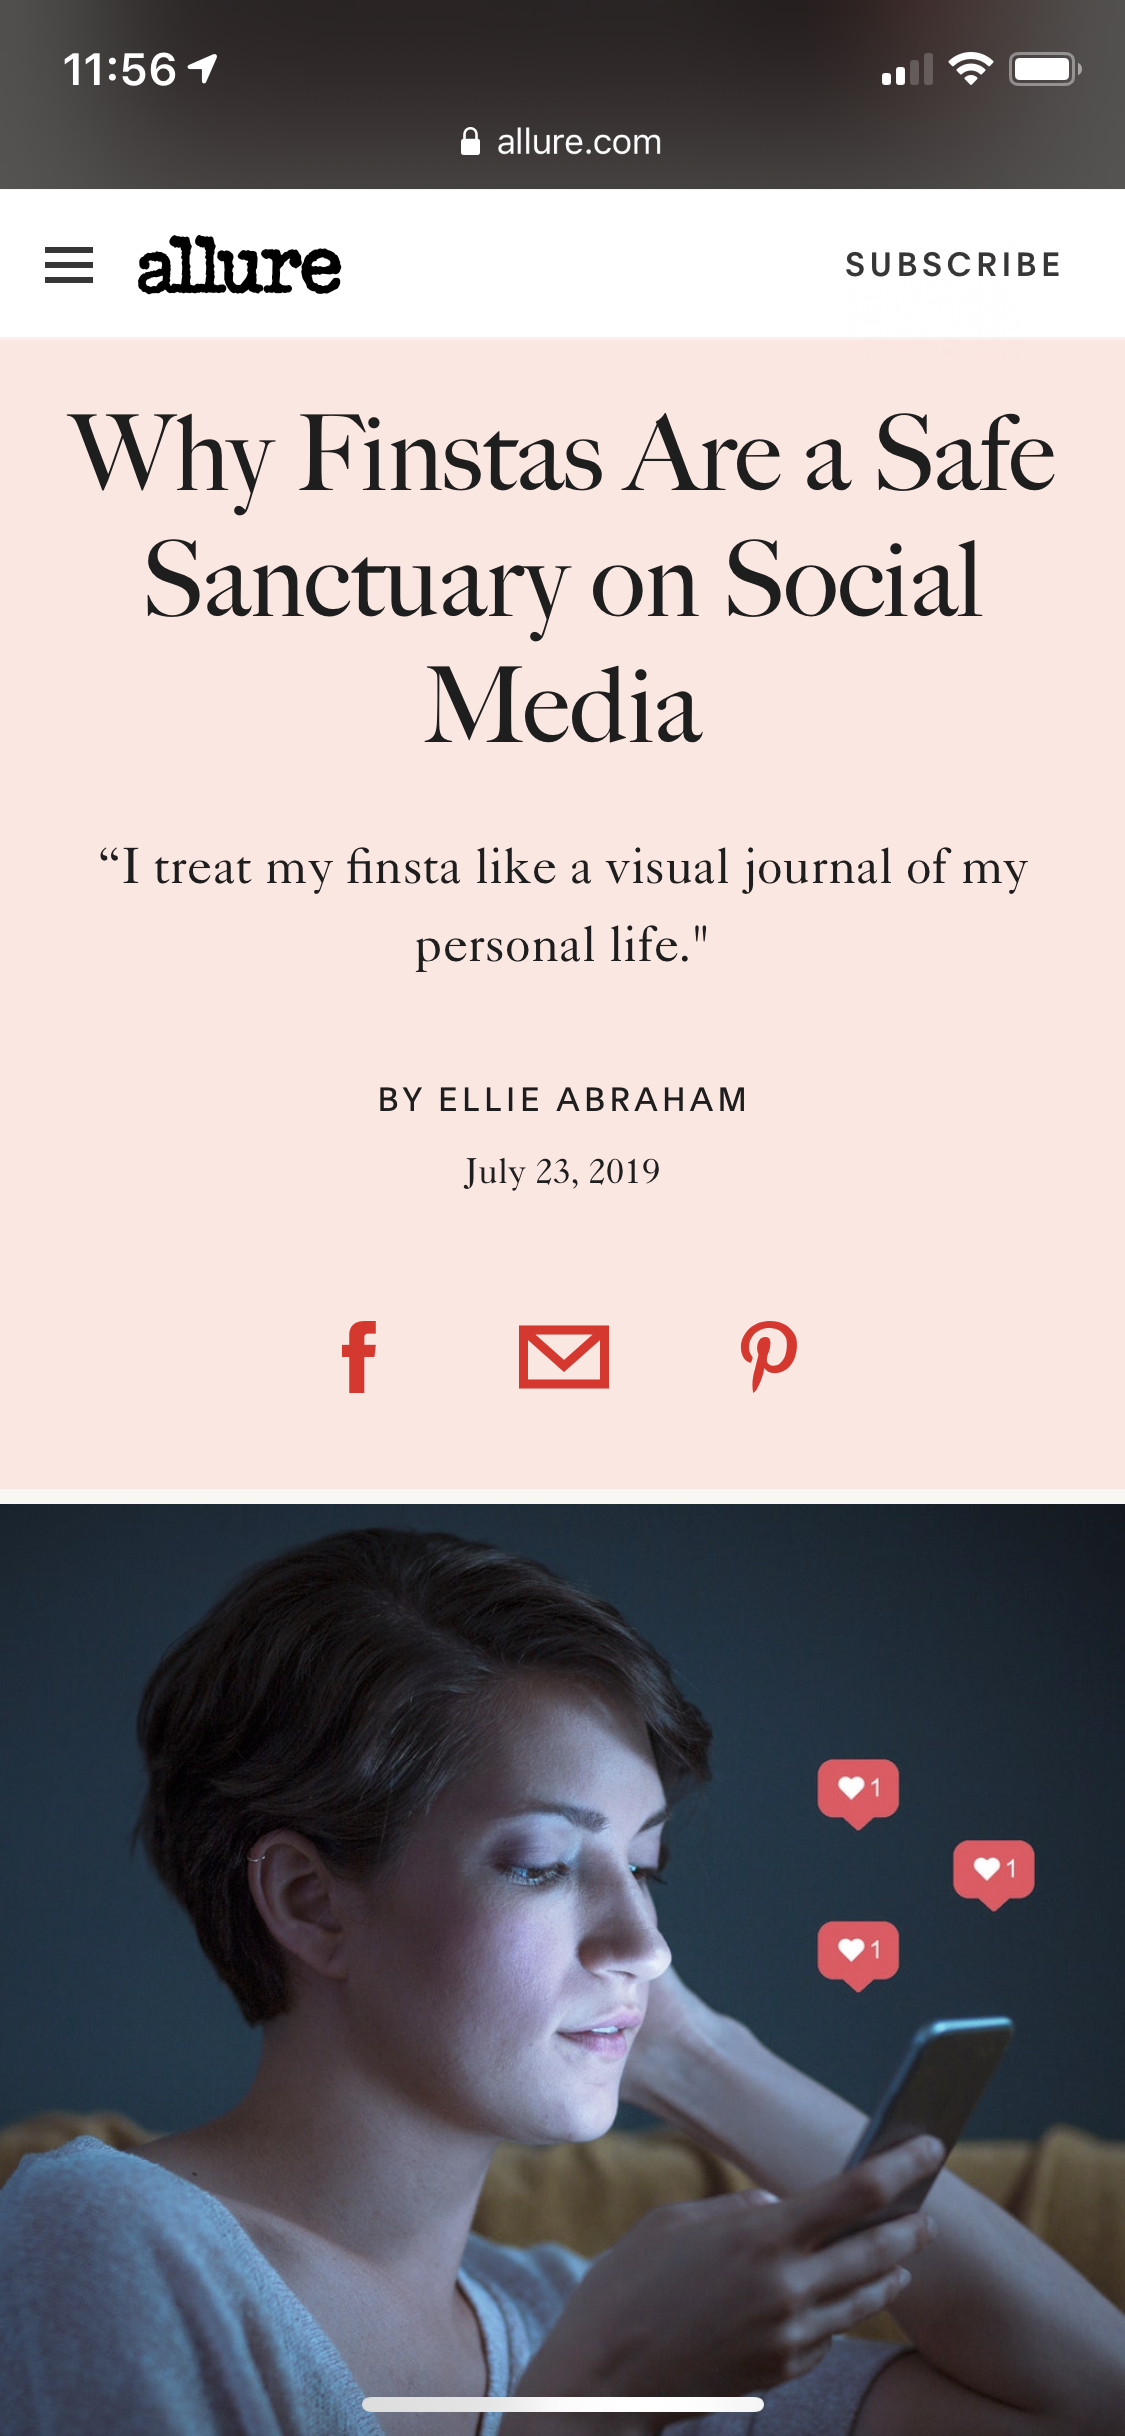
\includegraphics[width=0.4\textwidth]{figures/algo_hiding/IMG_4828}};}

      \visible<3->{\node [above right=-9cm and -0.5cm of img00] (img01) {\includegraphics[width=0.4\textwidth]{figures/algo_hiding/IMG_4830}};}
      
      \visible<4->{\node [below right=-8.5cm and -0.5cm of img01] (img02) {\includegraphics[width=0.4\textwidth]{figures/algo_hiding/IMG_4832}};}
  \end{tikzpicture}
  }
\only<6>{
\begin{center}
{\Large digital contact tracing}
\end{center}
}
\end{column}
\end{columns}
\end{frame}

\end{document}
